% THIS IS SIGPROC-SP.TEX - VERSION 3.1
% WORKS WITH V3.2SP OF ACM_PROC_ARTICLE-SP.CLS
% APRIL 2009
%
% It is an example file showing how to use the 'acm_proc_article-sp.cls' V3.2SP
% LaTeX2e document class file for Conference Proceedings submissions.
% ----------------------------------------------------------------------------------------------------------------
% This .tex file (and associated .cls V3.2SP) *DOES NOT* produce:
%       1) The Permission Statement
%       2) The Conference (location) Info information
%       3) The Copyright Line with ACM data
%       4) Page numbering
% ---------------------------------------------------------------------------------------------------------------
% It is an example which *does* use the .bib file (from which the .bbl file
% is produced).
% REMEMBER HOWEVER: After having produced the .bbl file,
% and prior to final submission,
% you need to 'insert'  your .bbl file into your source .tex file so as to provide
% ONE 'self-contained' source file.
%
% Questions regarding SIGS should be sent to
% Adrienne Griscti ---> griscti@acm.org
%
% Questions/suggestions regarding the guidelines, .tex and .cls files, etc. to
% Gerald Murray ---> murray@hq.acm.org
%
% For tracking purposes - this is V3.1SP - APRIL 2009

\documentclass{acm_proc_article-sp}

\usepackage{url}
\usepackage{wrapfig,lipsum}

% For roman numbers
\makeatletter
\newcommand*{\rom}[1]{\expandafter\@slowromancap\romannumeral #1@}
\makeatother
% For PHP code
\usepackage{listings,xcolor}
\definecolor{airforceblue}{rgb}{0.36, 0.54, 0.66}
\definecolor{dkgreen}{rgb}{0,.6,0}
\definecolor{dkblue}{rgb}{0,0,.6}
\definecolor{dkyellow}{cmyk}{0,0,.8,.3}

\lstset{
  language        = php,
  basicstyle      = \small\ttfamily,
  keywordstyle    = \color{dkblue},
  stringstyle     = \color{red},
  identifierstyle = \color{airforceblue},
  commentstyle    = \color{gray},
  emph            =[1]{php},
  emphstyle       =[1]\color{black},
  emph            =[2]{if,and,or,else},
  emphstyle       =[2]\color{dkyellow}}
  
%Fr JSON code
\colorlet{punct}{red!60!black}
\definecolor{background}{HTML}{EEEEEE}
\definecolor{delim}{RGB}{20,105,176}
\colorlet{numb}{magenta!60!black}

\lstdefinelanguage{json}{
    basicstyle=\normalfont\ttfamily,
    numberstyle=\scriptsize,
    stepnumber=1,
    numbersep=8pt,
    showstringspaces=false,
    breaklines=true,
    frame=lines,
    literate=
     *{0}{{{\color{numb}0}}}{1}
      {1}{{{\color{numb}1}}}{1}
      {2}{{{\color{numb}2}}}{1}
      {3}{{{\color{numb}3}}}{1}
      {4}{{{\color{numb}4}}}{1}
      {5}{{{\color{numb}5}}}{1}
      {6}{{{\color{numb}6}}}{1}
      {7}{{{\color{numb}7}}}{1}
      {8}{{{\color{numb}8}}}{1}
      {9}{{{\color{numb}9}}}{1}
      {:}{{{\color{punct}{:}}}}{1}
      {,}{{{\color{punct}{,}}}}{1}
      {\{}{{{\color{delim}{\{}}}}{1}
      {\}}{{{\color{delim}{\}}}}}{1}
      {[}{{{\color{delim}{[}}}}{1}
      {]}{{{\color{delim}{]}}}}{1},
}
\begin{document}

\title{Prototyping of a Browser-Based Social N-Screen Platform}
\subtitle{[Building Up to Boost User Experience]
}
%
% You need the command \numberofauthors to handle the 'placement
% and alignment' of the authors beneath the title.
%
% For aesthetic reasons, we recommend 'three authors at a time'
% i.e. three 'name/affiliation blocks' be placed beneath the title.
%
% NOTE: You are NOT restricted in how many 'rows' of
% "name/affiliations" may appear. We just ask that you restrict
% the number of 'columns' to three.
%
% Because of the available 'opening page real-estate'
% we ask you to refrain from putting more than six authors
% (two rows with three columns) beneath the article title.
% More than six makes the first-page appear very cluttered indeed.
%
% Use the \alignauthor commands to handle the names
% and affiliations for an 'aesthetic maximum' of six authors.
% Add names, affiliations, addresses for
% the seventh etc. author(s) as the argument for the
% \additionalauthors command.
% These 'additional authors' will be output/set for you
% without further effort on your part as the last section in
% the body of your article BEFORE References or any Appendices.

\numberofauthors{1} %  in this sample file, there are a *total*
% of EIGHT authors. SIX appear on the 'first-page' (for formatting
% reasons) and the remaining two appear in the \additionalauthors section.
%
\author{
% You can go ahead and credit any number of authors here,
% e.g. one 'row of three' or two rows (consisting of one row of three
% and a second row of one, two or three).
%
% The command \alignauthor (no curly braces needed) should
% precede each author name, affiliation/snail-mail address and
% e-mail address. Additionally, tag each line of
% affiliation/address with \affaddr, and tag the
% e-mail address with \email.
%
% 1st. author
\alignauthor
Bego\~na \'Alvarez de la Cruz\\
       \affaddr{Computer Science MSc Thesis}\\
       \affaddr{Web \& Media Group}\\
       \affaddr{Vrije Universiteit, Amsterdam}\\
       \email{begona.alvarezd@gmail.com}
}

% TO DO ABSTRACT---> LAST MORE OR LESS
\maketitle
\begin{abstract}
A second screen is a hand-device which is susceptible to provide added value to the TV content consumption. Notube, with their web browser-based second screen application, moved further through this concept, creating an assosiation between the second screen, Web and TV content. Nevertheless, the implemention still lacks completion in order achieve a full service and its users' satisfaction.

This project shows the development of a social N-Screen prototype based on previous researches and implementations carried out by Notube. This platform is intended to be used by small groups to explore on-demand content. The main goal of the project is consisted on searching and implementing features to the platform in order to offer to the final user an improved user experience. This improvement is leaded by the features that allow a completion in the user interaction flow with the platform, such as the implementation of a registration and login, the provision of persistence to the user based content and the addition of new functionalities as personal lists and likes/dislikes tracking.
\end{abstract}

\section{Introduction}

\subsection{Background}

\subsubsection{The Multi-Screen World}

The human being has become throughout the last years into a multi-screener\footnote{\textit{Multi-screening}: use of 
more than one screen at a time.} nation. From the appearance of television in our living rooms, until the incorporation of lighter and portable new devices such as smartphones or tablets, users have been including all these devices in their routines until turning them into everyday objects. Consequently, tablets, smartphones, televisions and computers have become the main group of devices with which an average user consumes most of their media content\cite{multiscreen:google}. 

\begin{figure}[!htb]
\centering
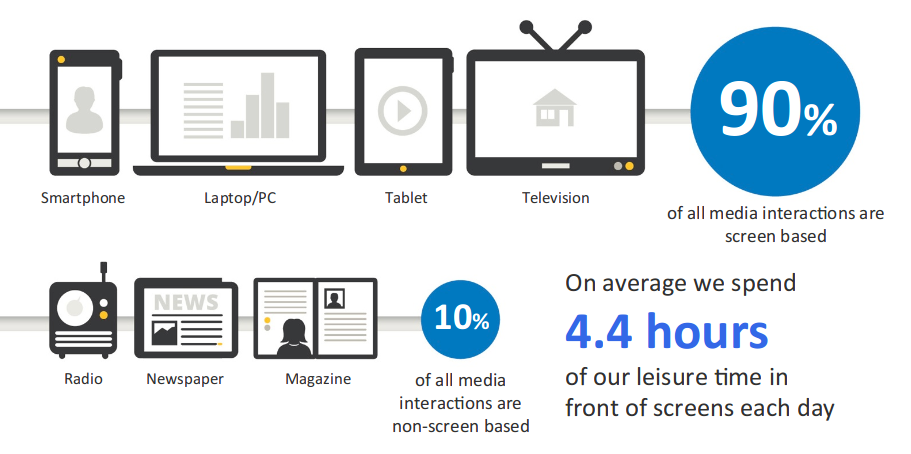
\epsfig{file=images/multiscreen-google.png, height=1.5in, width=3in}
\caption{Study of daily media interaction, obtained from \cite{multiscreen:google}}
\end{figure}

Despite each archetype provides a particular motivation and practise to users, an important fact is that screen devices as mentioned before are no longer used in isolation but collaboratively. Regarding this device collaboration, two different models of multi-screen\cite{multiscreen:google} behaviour are distinguished:  sequential and simultaneous. \textit{Sequential usage} refers to moving through more than one device in order to achieve a task. \textit{Simultaneous} concerns the usage of multiple devices at the same time for either related or unrelated activities. Both consumption forms are increasingly becoming the default mode and is surely influencing the way users engage. 

Following this scenario comes the necessity to understand how users interact with these screen devices in combination\cite{hritzuk2014multiscreen}. The opportunity to decide which device to use, where and how makes possible for users to control their own interaction and content flow. 

\begin{figure}[!htb]
	\centering
	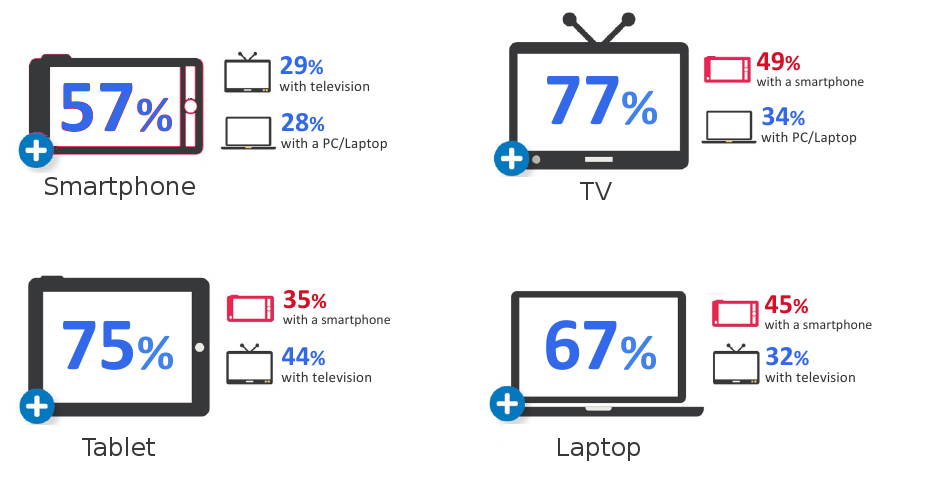
\epsfig{file=images/multi_usage2.png, height=2in, width=3.5in}
	\caption{Study of companion devices during simultaneous	 usage, obtained from \cite{multiscreen:google}}
	\label{fig:simultaneous}
\end{figure}

A Google study developed in 2012 \cite{multiscreen:google} exposed how an average consumer makes use of companion devices - smartphone, TV, tablet and laptop - during simultaneous\footnote{Usage for either related or unrelated activities.} usage - See Figure \ref{fig:simultaneous}. There are three main multi-screen combinations:
\begin{itemize}
  \item[-] Smartphone + TV\hspace{1.35cm}- 81\% 
  \item[-] Smartphone + Laptop/PC \hspace{0.1cm}- 66\% 
  \item[-] Laptop/PC  + TV\hspace{1.35cm} - 66\% 
\end{itemize}

Additionally, a research developed by Microsoft in 2013 \cite{microsoftcross} illustrated how is the user behaviour while multi-screening in simultaneous usage.  

\begin{itemize}
  \item[-] 68\% of consumers interact with multiple devices at the same time to access unrelated content; e.g. they may be texting a friend while watching TV. 
  \item[-] 57\% of consumers make use of more than one device simultaneously in order to achieve a related activity. 
\end{itemize}

From now on, we will focus our attention in simultaneous usage for \textit{related} activities.
 	
\subsubsection{Second Screens}

One of our everyday routines that has been altered by this new screen multitasking\cite{wiki:multitask}\footnote{\textit{'Human multitasking} is the apparent performance by an individual of handling more than one task at the same time.'} behaviour is that moment while a user watches TV. Viewers no longer focus their entire attention to the TV screen but share it with portable devices. 

\begin{figure}[!htb]
	\centering
	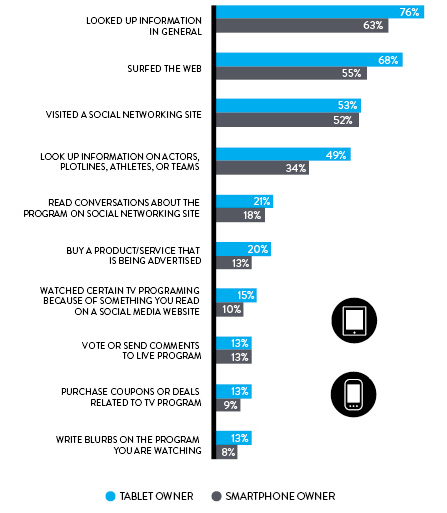
\epsfig{file=images/nielsen-tv-viewing.png, height=3.4in, width=3in}
	\caption{Tablet or smartphone activities while watching TV, obtained from \cite{nielsentv}}
	\label{fig:nielsengraph}
\end{figure}

Figure \ref{fig:nielsengraph} illustrates how consumers make use of their tablets and smartphones while watching TV. We can observe how indeed users not only surf on the web, but they interact with the device with activities directly related to the program or advertisement that they are watching at that moment. This demonstrates the fact that consumers are not merely interacting with their hand devices as a simple distraction, but sometimes in order to improve their TV content consumption. 

This new practice has led to the creation of the new concept \textit{second screen}. Second screen is a hand-device which is susceptible to provide added value to the TV content consumption. These devices such as tablets or smartphones play a role as companion
screens that 'connect' viewers to complementary interaction
opportunities while they watch TV via applications, additional
show-oriented content or in-synch functionalities \cite{evolumedia2}. 

This new activity has become such important that a survey developed by Nielsen Holdings N.V. \cite{nielsentv} reported 'Using a tablet or smartphone while watching TV is more common than not'. Nearly half of tablet owners - 43\%- and smartphone owners - 46\% - declared that while watching TV they are making use of their devices as second screen every day. As a consequence of this fact, there are emerging new apps\cite{wiki:app}\footnote{\textit{'App} is an abbreviation for application. An app is a piece of software. It can run on the Internet, on a computer, on a phone or other electronic device.'} which take advantage offering second screen experiences that can improve even more this interactivity while watching TV. 

Second screen apps \cite{evolumedia1} are intended to enable viewers to interact before, during and after the broadcast of a programme using a laptop, smartphone or tablet. The most competent apps, instead of distract, have the potential to increase the viewers' attention and enjoyment on the watching programme. According to \cite{evolumedia1}, eight types are distinguished in order to categorize these apps based on their functionalities: 
\begin{itemize}
  \item[-] Socializing
  \item[-] Loyalty
  \item[-] Recommendation
  \item[-] Transaction
  \item[-] Information
  \item[-] Program guides
  \item[-] Participation
  \item[-] Creation
\end{itemize}
On that account, second screen apps arised as a manner to unlock new research and business models due to the wide range of potential possibilities they offer. 

\subsubsection{Use case}

This project is based on an already existing platform developed by \textbf{Notube}\cite{aroyo2009notube}. Notube, is a project funded on 2009 that was specialized in second screens and Web merging. Their motivation was getting the Web and TV closer together via shared data models and content across multiple devices. They developed their own N-Screen\footnote{\textit{N-Screen} because it might be the primary screen, or one of a bunch of equals.} prototype, a Web browser-based\cite{business:bb}\footnote{\textit{'Browser-based} refers to computer tools and applications which run on a web browser via the Internet without accessing the operating system of any individual computer. These applications are accessed through web pages and can be used by people who are prevented from downloading software applications by firewalls.'} second screen application\footnote{All the source files used to generate this application can be accessed at the public repository:
\textit{https://github.com/notube/n-screen}} for small group exploration of on-demand content, both in the same room and remotely, with each individual having their own second screen device. It integrates different combinations of recommendation strategies and allows to decide within a closed group to watch a selected program sharing a 'virtual television', that in their case is the hand device itself. 

\begin{figure}[!htb]
	\centering
	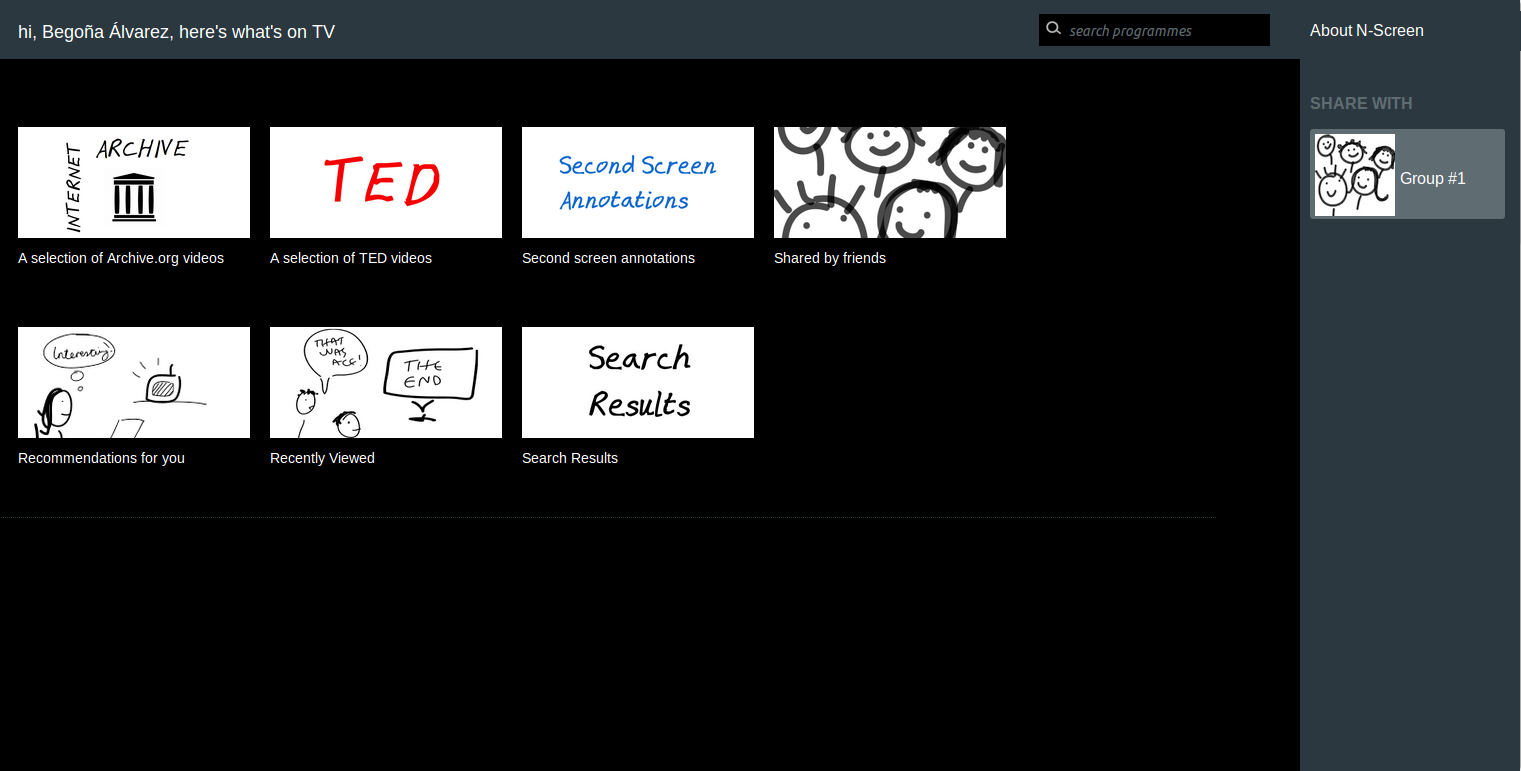
\epsfig{file=images/old_nscreen_screenshot.png, height=2in, width=3.3in}
	\caption{Notube N-Screen screenshot, source code obtained from the public repository \textit{https://github.com/notube/n-screen}}
	\label{fig:oldnotubenscreen}
\end{figure}

It is developed following a \textit{user-centric approach}\footnote{Placing user's goals at the heart of development.} in order to explore main aspects of users' content customisation demands, interaction requirements and entertainment preferences. Their main goal was to investigate if making decisions in collaboration might guide people to find something interesting to watch. 

\subsection{Goals}

The main goal of the project is to re-design, implement and improve the functionallity, interactivity and user experience of the browser-based second screen recommender platform\cite{tech:platform}\footnote{'A \textit{platform} is a group of technologies that are used as a base upon which other applications, processes or technologies are developed.'} carried out by Notube, in order to provide an attractive functional platform that can be used to graphically test different recommendation strategies. 

Most of the second screen apps in the market are not successfully developed because they are focused on enhance activities  that do not fulfil the real consumer needs\cite{evolumedia1}. Consequently, the audience engagement fails. This fact is crucial and it must be taken into account in order to make the platform valuable.

In addition, the platform must been design taking into account a possible future recommendation system integration. Furthermore, the project must accomplish certain requirements for a potential release to final users. It needs to be developed offering user-based content, due to its recommendation feature. It is required to provide engaging content and interaction activities, as well as offering an intuitive appearance. Moreover, the platform must be flexible and scalable, so it will not need to be entirely redone with every particular change. Hence, it is needed to reach a complete solution covering all these features, overcoming the gaps and deficiencies that other platforms show.

Here, the main goal is fragmented into more specific subgoals:

\begin{itemize}
  \item[-] \textit{Analysis of previous conclusions and results}. Study of already tested aspects. Definition of new tests to provide new data of interest. These data will help in making decisions about the implementation of interaction activities. 
  \item[-] \textit{Requirements definition}. Study of needs and constraints.
  \item[-] \textit{Software design}. Global design of the new involved software. Debugging and optimization.  
  \item[-] \textit{Platform development}. Implementation and integration in order to achieve the development of the final demo. 
  \item[-] \textit{General purpose tests}. Tests oriented to prove the proper operation and verify
the achievement of the requirements and constraints compliance.
  \item[-] \textit{Results analysis and conclusions}. Achievement evaluation. Study of weaknesses or possible improvements. Definition of further studies.
\end{itemize}

\subsection{Project Organization}
The organization of this project is described as follows:
\begin{itemize}
  \item \textit{Analysis of previous conclusions and results}. 
  
  At this first stage, N-Screen-related information and specific knowledge was acquired. An approach to the development tools was also outlined. Goals:
  \begin{itemize}
  	\item [-]Second screen state-of-the-art review. Review of the current commercial
solutions.
	\item [-]Adaptation to the development of the platform as well as required tools (repository, client and server side programming languages research and learning, etc\dots).
	\item [-]Analysis of related projects results, either completed or under development. 
  \end{itemize}
  
  \item \textit{Software design}.
  
  This phase covered from the first software definitions and  specifications, to the platform implementation until reaching a final demo. Goals:

  \begin{itemize}
  	\item [-]Software design and implementation for required features.
	\item [-]Content dataset migration. 
	\item [-]\textit{Alpha}-version deployment. Source code
debugging and improvement.
	\item [-]\textit{Beta}-version deployment. Source code
debugging and improvement.  
  \end{itemize}
	
  \item \textit{Tests and evaluation}. 
  
  At last, the final demo was evaluated and the results were analyzed. Goals:
  
  \begin{itemize}
  	\item [-]Technical Test.
	\item [-]User experience test.
	\item [-]Results interpretation and conclusions review. Statement of further studies and future development lines. Found problems evaluation.
  \end{itemize}
  
  \item \textit{Documentation generation}.
  
  Dissertation and other required documentation writing. 
\end{itemize}


\subsection{Outline}
Typically, the body of a paper is organized
into a hierarchical structure, with numbered or unnumbered
headings for sections, subsections, sub-subsections, and even
smaller sections.  The command \texttt{{\char'134}section} that
precedes this paragraph is part of such a
hierarchy.\footnote{This is the second footnote.  It
starts a series of three footnotes that add nothing
informational, but just give an idea of how footnotes work
and look. It is a wordy one, just so you see
how a longish one plays out.} \LaTeX\ handles the numbering
and placement of these headings for you, when you use
the appropriate heading commands around the titles
of the headings.  If you want a sub-subsection or
smaller part to be unnumbered in your output, simply append an
asterisk to the command name.  Examples of both
numbered and unnumbered headings will appear throughout the
balance of this sample document.


\section{State-of-Art}
Typically, the body of a paper is organized
into a hierarchical structure, with numbered or unnumbered
headings for sections, subsections, sub-subsections, and even
smaller sections.  The command \texttt{{\char'134}section} that
precedes this paragraph is part of such a
hierarchy.\footnote{This is the second footnote.  It
starts a series of three footnotes that add nothing
informational, but just give an idea of how footnotes work
and look. It is a wordy one, just so you see
how a longish one plays out.} \LaTeX\ handles the numbering
and placement of these headings for you, when you use
the appropriate heading commands around the titles
of the headings.  If you want a sub-subsection or
smaller part to be unnumbered in your output, simply append an
asterisk to the command name.  Examples of both
numbered and unnumbered headings will appear throughout the
balance of this sample document.


\section{Review Study}
A model for the platform is defined in this chapter. Initially, the first version of the N-Screen developed by Notube\cite{aroyo2009notube} is evaluated to obtain some guidelines and potential improvements facing our own. The final software implementation requirements and constraints are defined. Finally, a discussion and evaluation over different features is carried out, exposing different options and some final conclusions in order to face a potential deployment to final users.
\subsection{Browser-Based Social N-Screen Platform Model}

Essentially, the BBSNSP\footnote{Browser-Based Social N-Screen Platform} responds to a second screen application based on a recommendation system. However, a further review shows some general differences:

\begin{itemize}
  	\item [-]\textit{Browser-based}: instead of being developed as a mobile or computer app, the BBSNS is a web app. A \textit{web app} refers to software that runs on a web browser. This way, not only the app can be updated and maintained without disturbing potential users by requiring them to re-download. Additionally, it provides implicit support for cross-platform\cite{web:cp}\footnote{\textit{'Cross-platform} regards the capability of a software to run identically on different platforms.'} compatibility. 
	\item [-]\textit{Group decision recommendation system -Social-}. The recommendation feature is focused on 'how collaborating together might help people find something interesting to watch'\footnote{https://notube3.wordpress.com/2011/10/10/n-screen-a-second-screen-application-for-small-group-exploration-of-on-demand-content/}. It is designed to be used within a small group of friends in a collaboratively way to reach together a successful programme to watch. 
	\item [-]\textit{Apart\footnote{Different physical locations.} group oriented}: this BBSNS is mainly designed to watch together with other friends but being remotely located. 
	\item [-]\textit{N-Screen}: It is not only oriented to be used as a secondary. It is considered that it might be used as a primary screen, secondary screen, or one of a screen devices collection. 
\end{itemize}

\subsection{First Browser-Based Social N-Screen Platform Review} \label{firstNScreen}

The first BBSNSP was a project of Notube developed in 2011. It supposed a big step forward to get the Web and TV closer together using shared data models and content across multiple devices\cite{schopman2010notube}. It is designed to help deciding and enabling to interact using drag and drop over screen devices. It allowed to investigate  how helpful is group collaboration in order to find an interesting programme to watch, for limited group of users. It gave the strengths and weaknesses to establish the fundamentals for future developments.

While constituting a successful platform meeting most of its features, the Notube BBSNSP introduced some issues found after its evaluation. This issues are following listed. 

\rom{1}) As a recommender system, the platform is intended to be user based content oriented. User preferences and explicit interaction should provide to the recommendation strategies an on-real-time update to re-rank the displayed personal suggestions\cite{libbyrecommender}. In Notube's platform, user interaction is treated as \textit{volatile} data, each time that the session is closed, the information is lost. This implementation impedes to exploit all this relevant information. Figure\ref{fig:recomm} shows the 5 tasks that are intended to be accomplished by the recommendation engines in the client-side. If the platform lacks tracking the user interaction and preferences, it would not be possible to realize properly the first \textit{traing} step due to a shortcoming information.

\begin{figure}[!htb]
\centering
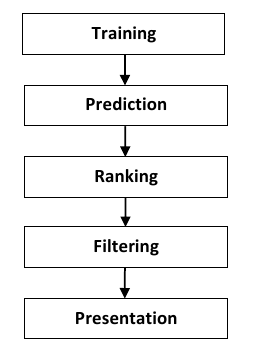
\epsfig{file=images/recommender_tasks.png, height=2in, width=1.5in}
\caption{Recommender system tasks, obtained from \cite{libbyrecommender}}
\label{fig:recomm}
\end{figure}

\rom{2}) Their own preliminary findings after the evaluation\footnote{https://notube3.wordpress.com/2011/12/12/preliminary-findings-of-n-screen-user-testing/} showed us a weak point. Notube results obtained after testing N-Screen with real users showed how some of them received a successful recommendation and indeed were wishing to watch later that specific selected programme. They received feedback such as ''Not for watching something instantly, only for making suggestions for things that could choose to watch later if you wanted to'' or ''I do not think it is on to recommend things for others to watch instantly''. This results revealed an interesting \textit{sequential usage} behaviour. In this case, instead of passing from one device to another, the user is making use of the same device time later to accomplish a task. Therefore, not only the volatile activity of the user, but also a lack of option to save wished programmes for a future moment, makes unlikely the activity to watch \textit{that programme later}. 

\rom{3}) It is very important to offer an attractive set of possible activities for the user to interact with the \cite{skadberg2004visitors}. The only implicit offered interactions are the browsing and the suggestion part. For this reason, we found that Notube N-Screen slightly incomplete in terms of interactivity actions. 

\rom{4}) The platform was designed to be not only a recommendation system, but also a place to watch a selected programme. There exist two different ways to realize this action: locally and remotely. 
The first one is performed when a user decides to watch a programme individually. By contrast, the second one is conducted when a group decides to watch together a selected programme and the members are located in remote locations. This last visualization mode involves the execution of a browser-based 'virtual TV' in which every person within the group can watch simultaneously the same. Unfortunately,  this last feature was not working because the programme visualization part was missing. Making the virtual TV feature working is indeed necessary for a complete success of the platform. 

\rom{5}) As mentioned before in this section, issue \rom{1}), the platform is designed to provide -future- recommendation strategies. For this purpose, its  structure design needs to be flexible and scalable to allow future recommendation scripts compatible in terms of data, in this case, a wide set of programmes. Following a deep study of the source code, we found and important bottleneck. The implementation was not flexible to face data content migrations. The programmes displayed, and all the logic behind it, were designed to correctly work just locally and with a limited flexibility range. It is not possible to afford heavy data as a wide set of programmes running locally due to memory limitations. 


\rom{6}) The inherit second screen behaviour of the platform makes strongly important to take into account that higher complex interaction in this type of environments is a determinative factor \cite{cruickshank2007making}, since involves a multi-tasking activity. We found that the homepage was not simple while informative enough in order to not distract the user from the main screen attention. It lacked first sight relevant information, therefore it required more attention than actually needed. 

\section{Implementation Study}
Once the first BBSNSP has been reviewed, it is moment to study how to settle every found issue and bottleneck exposed in Section \ref{firstNScreen} and start the implementation. The decisions regarding the implementation of new features are exposed. 

\subsubsection{Localhost Deployment}

Before being able to start programming the platform, it was required preparing the environment. 

On the one hand, it was needed to set up a local server to be able to run and test our web application. We used XAMPP on a Linux distribution for this purpose, due to its multiple advantages and intuitiveness. XAMPP is an open source independent server platform which consists mainly of a MySQL database, Apache Web server and required interpreters for scripting languages as PHP and Perl. 

On the other hand, the set-up required an Ejabberd installation to manage instant messages in order to enable automatic non-typed communication between remote users and allow them to collaborate -suggest-. Ejabberd is a Jabber/XMPP\cite{wiki:xmpp}\footnote{\textit{'Extensible Messaging and Presence Protocol}, better known as XMPP (formerly Jabber), is an open and extensible XML-based protocol originally designed for instant messaging.'} server \cite{jia2010xmpp} which is realized in Erlang\footnote{Therefore, it was required also the Erlang packages installation for compilation} language. Its main functionality is that it works as an instant messaging server that allows more than one poeple to communicate and participate in real time, based on typed text or not. Additionally, considering that is intended to be used by a web application as part of a communication tool, it was necessary to enable BOSH in our Ejabberd server configuration. HTTP is synchronous providing simple call and response methods, discordant to XMPP's asynchronous event based protocol. Therefore, BOSH\footnote{Bidirectional-streams Over Synchronous HTTP} is a protocol that provided us a method to use XMPP in our platform by making http requests with a long time-out.

After this preparation, the environment was therefore ready to start the implementation. 
\subsection{Registration \& Login}

The platform is intended to be used to test researches developed about recommendation strategies, therefore, it follows a user content based model. As explained in Section \ref{firstNScreen} issue \rom{1}), user preferences and explicit interaction should provide to the recommendation strategies an on-real-time update to re-rank the displayed personal suggestions. In order to deal with the volatile data it was decided to implement a Registration \& Login system. This way, it is possible to tack user preferences and provide relevant data to the recommendation side. 

An important step before implementing the registration system was to study different types of registration which we could offer. Due to the imminent growth of the social networks popularity such as Facebook\footnote{https://www.facebook.com/} \cite{shih2009facebook}, websites are currently offering two different options to accomplish a registration:

\begin{itemize}
  	\item [-]\textit{Good registration}: known as the one where a user fills in directly the registration form with their personal data. 
	\item [-]\textit{OpenID}: OpenID Registation is an extension to the OpenID\cite{w3c:openid}\footnote{'OpenID is an interoperable authentication protocol designed to be safe, faster and easier way to log in to web sites.'} Authentication protocol that allows for very light-weight profile (mostly social networks profile, as Facebook or Twitter\footnote{https://www.twitter.com/}) exchange . It is designed to pass eight commonly requested pieces of information when an end user goes to register a new account with a web service. 
\end{itemize}\begin{figure}[!htb]
\centering
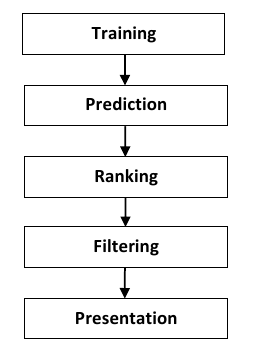
\epsfig{file=images/recommender_tasks.png, height=2in, width=1.5in}
\caption{Recommender system tasks, obtained from \cite{libbyrecommender}}
\label{fig:recomm}
\end{figure}

The OpenID provides an even faster registration than before. This '1-click' activity can definitely be very attractive to implement as unique registration for a second screen platform\cite{allen2012smashing}, where users distraction has a crucial importance. But despite its significance through the last years, not every user is willing to share their social networks' personal profile due to a lack of confidence in such websites\cite{pu2006trust}. For this reason, we decided to include both in our platform, selecting the OpenID registration provided by Facebook, since this social network can offer valuable information for the recommendation system. 


The implementation for registration \& login has been carried out making use of:

\begin{itemize}
  	\item \textit{MySQL database}
	\item \textit{Database handler scripts}: 
	\begin{itemize}
  		\item [-]HTML5 submit forms \& PHP for the good registration 
		\item [-]Javascript Facebook SDK\cite{web:sdk}\footnote{\textit{'Software Development Kit} (SDK) refers to a programming package that enables a programmer to develop applications for a specific platform.'} \& PHP for the OpenID registration 
	\end{itemize}
\end{itemize}

\subsubsection{Database}

The structure of our database has been changing as the platform evolved. At the end, intending to match every needed requirement, we reached the following schema based on two tables:

Table \texttt{members}. Column fields:

\begin{itemize}
\item \texttt{member\_id}: Primary key\footnote{The \textit{primary key} of a relational table uniquely identifies each record in the table.}
\item \texttt{firstname}: First Name
\item \texttt{lastname}: Last Name
\item \texttt{login}: Unique user-name
\item \texttt{passwd}: MD5 encrypted\cite{wiki:md5}\footnote{'The \textit{MD5} message-digest algorithm is a widely used cryptographic hash function producing a 128-bit (16-byte) hash value, typically expressed in text format as a 32 digit hexadecimal number.'}
\item \texttt{facebook\_id}: unique ID extracted from Facebook OpenID.
\end{itemize}

Table \texttt{content}. Column fields:

\begin{itemize}
\item \texttt{member\_id}: Primary key\footnote{The \textit{primary key} of a relational table uniquely identifies each record in the table.}
\item \texttt{recommendations}: Personal recommendations list, JSON\footnote{\textit{'JSON} (JavaScript Object Notation) is a lightweight format that is used for data interchanging.'} format.
\item \texttt{recently\_viewed}: Recently viewed or watched programmes personal list, JSON format.
\item \texttt{watch\_later}: Watch Later personal list, JSON format.
\item \texttt{like\_dislike}: List containing personal likes and dislikes of the user, JSON format.
\item \texttt{shared\_by\_friends}: List containing suggestions to the user made by members within his/her same group. 
\end{itemize}

For further details in terms of database fields definition, the following code (\texttt{mysql.sql}) shows in SQL language our tables initialization: 

\begin{lstlisting}[language=json,firstnumber=1]
CREATE TABLE IF NOT EXISTS `members` (
 `member_id` int(11) 
    unsigned NOT NULL AUTO_INCREMENT,
 `firstname` varchar(100) DEFAULT NULL,
 `lastname` varchar(100) DEFAULT NULL,
 `login` varchar(100) NOT NULL DEFAULT '',
 `passwd` varchar(32) NOT NULL DEFAULT '',
 `facebook_id` bigint(11) DEFAULT NULL,
 PRIMARY KEY (`member_id`)
) ENGINE=MyISAM  
    DEFAULT CHARSET=latin1 AUTO_INCREMENT=1 ;

CREATE TABLE IF NOT EXISTS `content` (
 `member_id` int(11) 
     NOT NULL AUTO_INCREMENT,
 `recommendations` longtext NOT NULL,
 `recently_viewed` longtext NOT NULL,
 `watch_later` longtext NOT NULL,
 `like_dislike` longtext NOT NULL,
 `shared_by_friends` longtext NOT NULL,
 PRIMARY KEY (`member_id`)
) ENGINE=InnoDB  
    DEFAULT CHARSET=latin1 AUTO_INCREMENT=1 ;
\end{lstlisting}

Picture whatever shows how the content is initialize for each user the very first moment during the registration. 

****INCLUDE AN IMAGE OF THE DATABASE STRUCTURE BEING POSTED BY REGISTRATION******

\subsubsection{Login Security}

An important implementation to mention is that, in order to access to the personal webpage after the login action, a security checking has been implemented. The access to the welcome page containing personal user-based content is only possible if the login has been correctly done, case in which the authentication \texttt{SESSION VARIABLES}\cite{php:session}\footnote{'A\textit{Session Variable} is an associative array containing session variables available to the current script.'} are set and authenticated. 

The following script (\texttt{auth.php}) shows this implementation:\footnote{\texttt{SESS\_MEMBER\_ID} is only initialized when the login authentication had been successful.}

\begin{lstlisting}[language=json,firstnumber=1]
<?php
//Start session
session_start();
	
//Check whether the session variable 
//SESS_MEMBER_ID is present or not
if(!isset($_SESSION['SESS_MEMBER_ID']) 
  || (trim($_SESSION['SESS_MEMBER_ID'])=='')){
  header("location:index.html");
  exit();
}
?>
\end{lstlisting}

In addition, for localhost testing purposes, it has been included a management of the browser cache to allow more than one sessions running simultaneously in the same browser.

\subsection{Interaction Activities}
\subsubsection{Watch Later} \label{watchlater}
It is severely important to understand how is the user behaviour when interacting with a web service. Developers and designers work together to deploy a final product, but sometimes users can present unpredictable conduct and wishes\cite{norman2002design}. It is only after realizing tests on final users when the success or failure can be declared. Notube N-Screen, for example, was designed to be a second screen recommendation platform to watch immediately a selected programme. But after a evaluation with real users they found out how some users where wishing to watch that successful recommended programme not immediately, but in another later moment. This result revealed a very interesting \textit{sequential usage} behaviour in which users utilize the same platform -and sometimes the same device- but in separated moments to accomplish a task, in this case, watch the desired programme. The platform therefore showed a general successful feedback, but was lacking an important user conduct that was not taking into account at the beginning. 

Our simplest and effective solution to this situation\cite{krug2014don} has been the implementation of the possibility to add programmes to a personal '\textit{watch later}' list. This list is directly populated with the implicit user interaction of clicking a 'watch later' button. The list can be edited by the addition or removal of a programme. It is important to mention that each time the user edits this personal list, it is directly updated in the database making use of the PHP script \texttt{set\_channel.php}, which source code is as follows:

\begin{lstlisting}[language=json,firstnumber=1]
<?php
 //Start session
 session_start();
 $data = mysql_escape_string($_POST['data']);
 $channel = $_POST['channel'];
 ini_set( 'default_charset', 'UTF-8' );
	
 //Include database connection details
 require_once('config.php');

 //Connect to mysql server
 $link = mysql_connect(DB_HOST, DB_USER, DB_PASSWORD);
 if(!$link) {
  die(''Failed to connect to server:''.mysql_error());
 }
	
 //Selecting database for the user
 $db = mysql_select_db(DB_DATABASE);
 if(!$db) {
  die(''Unable to select database'');
 }
 $member_id = $_SESSION['SESS_MEMBER_ID'];

 mysql_query(''UPDATE content SET $channel = 
   '$data' WHERE member_id = '$member_id''');
?>
\end{lstlisting}

****INCLUDE SCREENSHOT WATCH LATER ******

\subsubsection{Like \& Dislike}
As mentioned in Section \ref{firstNScreen} issue \rom{3}), we analysed Notube N-Screen and we found that the platform was missing interaction activities. The implementation of the Watch Later list explained in Section \ref{watchlater} is  actually an addition that improves this issue. Nevertheless, after a deep study we came to the result that just adding that feature was not enough. Based on the recommendation system that is going to be included afterwards, we converged to an idea to include the possibility to elicit user preferences by ranking a programme with a simple Like or Dislike action. 

The idea came from the project developed by Vista-TV Sibyl\footnote{http://sibyl.prototyping.bbc.co.uk/}. Sibyl is a TV and radio programme recommender system designed for tablets and personal computers which uses a novel drag-and-drop system to extract user preferences. A user is able to express preferences by dragging individual programmes into 'like' and 'dislike' boxes. These preferences are immediately used by the client-side recommender to re-rank the programmes and refresh the recommendation list. Therefore, the implementation in N-Screen not only improves the user interaction, but also can be used to improve the recommendation strategy using directly relevant information provided by the user. 

As well as with the case of the Watch Later list, likes and dislikes are directly populated with the implicit user interaction of clicking a button; simultaneously updating the database with PHP script \texttt{set\_channel.php}. 

*****PONER IMAGEN DE LIKES AND DISLIKES*******

\subsubsection{Hyperlink Metadata}

In order to keep improving the platform without distracting the user from the main purpose\cite{allen2012smashing} that is watch a programme, we decided to implement another more additional feature: Hyperlin\cite{wiki:hyper}\footnote{\textit{'Hyperlink} is a reference to data that the reader can directly follow either by clicking or by hovering or that is followed automatically.'} Metadata\footnote{\textit{Metadata}: data about data. It is descriptive information about a particular data set, object, or resource.}. Inside each selected programme description, we included the possibility to click hyperlink metadata to browse further information of this selected concept. The first idea was to add the possibility to include clickable actions to actor, director, genre and general metadata of a TV programme. Unfortunately, it has been only possible to implement the hyperlink with 'tags'  due to content dataset restrictions - data explanation in Section \ref{data}-. For that reason it has been possible only to display only a small part of the goal, but the implementation is developed to work successfully with other datasets that provide wider content extraction.

****PONER IMAGEN DE POSIBILIDAD DE CLICKAR METADATA****

\subsubsection{Random Selection}

\subsection{Remote TV}

Social activities through the Web are becoming exponentially popular since the web encourages users to  participate socially active without even moving from their rooms\cite{schopman2010notube}. On the other hand, TV remains a largely passive experience that usually requires physical presence to become social in terms of simultaneous experience sharing, i.e. if you want to watch the same programme al the same time with a friend, you usually meet together in order to do it. For this reason, one of the most innovative and attractive features included in Notube N-Screen was the possibility to share a cross-platform 'virtual TV' in which every person within a group can watch simultaneously the same. Watching TV with faraway friends through a virtual living room.

Unfortunately, as explained in \ref{firstNScreen} issue \rom{4}), this last feature was not working because the programme visualization part was missing. We decided that it was necessary to resuscitate the virtual television in order to achieve a successful platform. After long time studying the source code \texttt{player.html}, the bug was found. The problem was mainly residing in data compatibility and how \texttt{player.html} handled this data to enable a visualization. Further details concerning data structure are explained in section \ref{data}. The following \texttt{player.html} section of code shows how we handled the issue, replacing the local '\textit{manifest}'\footnote{The \textit{manifest} provides relevant  metadata for a specific programme such as video-url and video-format} extraction for a \texttt{http-request} in order to retrieve the manifest, and therefore, fixing the problem. 
\begin{lstlisting}[language=json,firstnumber=1]
$(document).bind('tv_changed', function (e,item) {
  console.log(item);
  var programme = item.nowp;
  var id =  item.nowp.id;
  me.nowp = item.nowp;
  $("#title").html(programme["title"]);

  var action = "Play";
  if(programme && programme["action"]){
        action = programme["action"];
  }  
  show_message(action+'ing'+programme["title"]);

  if(action=="Play"){

  $.ajax({
    url: "get_tedtalks_by_id.php",
    type: "POST",
    async: false,
    data: {id: id},
    dataType: "json",
    success: function (data) {
      item =  changeData(data); 
      //JSON with suggestions format
      var manifest = item.suggestions[0].manifest;
      process_manifest(manifest,programme);
    }
  });
  // ---- PREVIOUS CODE -----
  //pretty much everything should have a manifest
    // var manifest = programme["manifest"];
    // var manifest = item.manifest;
    // if(manifest){
    //   console.log("manifest is "+manifest);
  
    //     $.ajax({
    //     url: manifest,
    //     dataType: "json",
    //     success: function(data){
    //      process_manifest(data,programme);
    //      }
    //     }); 
   }else{
     alert(''no manifest'');
   }
});
\end{lstlisting}

*******PONER IMAGENES QUE DEMUESTRAN EL FUNCIONAMIENTO DE LA REMOTE****
\subsection{Content Data} \label{data}
This project presents a functional platform that can be used, between others, to test future recommendation strategies. One of the possibilities that are currently being researched in our Web \& Media Department \footnote{http://wm.cs.vu.nl/} is a recommendation system based on BBC\cite{wiki:bbc}\footnote{\textit{'British Broadcasting Corporation} (BBC) is a UK-based international public-service broadcaster head-quartered at Broadcasting House in London.'} programmes through the webpage \texttt{http://www.bbc.co.uk/programmes/}. As mentioned in section \ref{firstNScreen} issue \rom{5}), the Notube N-Screen structure was designed to work with locally stored data. This approach was inefficient since facing future data migrations or including heavier data would follow not only memory but also functional issues. Consequently, we decided to change how the platform deals with this. We converted it to a platform structure designed to deal with remotely stored data based on programmes' IDs including metadata extraction. In order to make this happen, a set of scripts to handle \texttt{http-requests}\footnote{ \textit{HTTP request/response} protocol, which means a client-side application sends a request for some file, and the web server sends back a response.} has been implemented. These scripts have been programmed making use of Javascript\cite{w3c:ajax}\footnote{\textit{'Asynchronous JavaScript and XML} (AJAX) is the method of exchanging data with a server, and updating parts of a web page without reloading the entire page.'} AJAX in the client side, and PHP in the server side. This way, it is not needed to locally store testing datasets but to provide to the scripts a suitable URL to extract information. As a result, the functionality speed is maintained at the same time the platform total weight is severely reduced, since it does not locally store any dataset. 

In addition, it has been taking into account the possible data structure that the recommendation system may use as input. For this purpose, a deep study of data structure compatibility has been conducted to facilitate as much a possible future implementations carried out by recommendation engines researchers. Based on various data extraction APIs\footnote{\textit{Application-Programming Interface}} such as the \textit{BBC Developers API}\footnote{https://developer.bbc.co.uk/} or the \textit{TED Talks Lab API}\footnote{http://developer.ted.com/API\_Docs}
we decided to set up the following structure\footnote{Notice that it is a random example using a extracted TED Talks Video.} in \texttt{JSON} format for every object contained in our N-Screen, as programmes or videos:
\begin{lstlisting}[language=json,firstnumber=1]
{
"pid":1000,
"title":"Gero Miesenboeck: Re-engineering the brain",
"description":"In the quest to map the brain, many scientists have attempted the incredibly daunting task of recording the activity of each neuron. Gero Miesenboeck works backward -- manipulating specific neurons to figure out exactly what they do, through a series of stunning experiments that reengineer the way fruit flies percieve light.",
"date_time":"2010-11-03 22:44:00",
"url":"http://download.ted.com/talks/GeroMiesenboeck_2010G-950k.mp4",
"video":"http://download.ted.com/talks/GeroMiesenboeck_2010G-950k.mp4",
"speaker":[
{
"speaker":{
   "id":741,
   "title":"",
   "firstname":"Gero",
   "middleinitial":"",
   "lastname":"Miesenboeck",
   "description":"Optogeneticist",
   "whotheyare":"Using light and a little genetic engineering -- optogenetics -- Gero Miesenboeck has developed a way to control how living nerve cells work, and advanced understanding of how the brain controls behavior.",
   "whylisten":"<p>Gero Miesenboeck is pioneering the field of optogenetics: genetically modifying nerve cells to respond to light. By flashing light at a modified neuron in a living nervous system, Miesenboeck and his collaborators can mimic a brain impulse -- and then study what happens next. Optogenetics will allow ever more precise experiments on living brains, allowing us to gather better evidence on how electrical impulses on tissue translate into actual behavior and thoughts...</p>",
   "slug":"gero_miesenboeck",
   "published_at":"2010-06-09 08:14:00",
   "updated_at":"2010-11-04 15:11:51"
}
}
],
"image":"http://images.ted.com/images/ted/51f652b9ff6854867d1d7abb2683caf1d8dd22fb_240x180.jpg",
"manifest":{
"pid":1000,
"id":1000,
"title":"Gero Miesenboeck: Re-engineering the brain",
"image":"http://images.ted.com/images/ted/51f652b9ff6854867d1d7abb2683caf1d8dd22fb_240x180.jpg",
"provider":"ted",
"duration":1750,
"media":{
"mp4":{
   "uri":"http://download.ted.com/talks/GeroMiesenboeck_2010G-950k.mp4",
   "is_live":"false"
}
},
"type":"video/mp4"
},
"tags":{
"biology":"biology",
"brain":"brain",
"neurology":"neurology",
"science":"science"
}
},
\end{lstlisting}

In order to parse every possible response provided by the API selected to extract videos and programmes collection, it has been implemented a JavaScript function to set up a total compatibility in our platform. This script is named \texttt{changeData(data)} which source code is as follows:

\begin{lstlisting}[language=json,firstnumber=1]
//Adapt any http request to our own data format

function changeData(data){

  var random_ted = {
    suggestions: []
  };

  if(data.talks == null){
    return random_ted;
  }  

  for(var i = 0; i < data.talks.length; i++) {  var item = data.talks[i];
      for(var j = 0; j < data.talks[i].talk.photo_urls.length; j++){
        if(data.talks[i].talk.photo_urls[j].size == "240x180"){
          var image = data.talks[i].talk.photo_urls[j].url;
        }
      } 

      if(item.talk.media_profile_uris["internal"]){

      random_ted.suggestions.push({ 
          "pid"   : item.talk.id,
          "title" : item.talk.name,          
          "description" : item.talk.description,
          "date_time" : item.talk.published_at,
          // "media_profile_uris" : item.talk.media_profile_uris,
          "url" : item.talk.media_profile_uris["internal"]["950k"].uri, //TODO CHANGE THIS
          "video" : item.talk.media_profile_uris["internal"]["950k"].uri,
          "speaker" : item.talk.speakers,
          "image" : image,
          "manifest" : {
              "pid"   : item.talk.id,
              "id" : item.talk.id,          
              "title" : item.talk.name,
              "image" : image,
              "provider" : "ted",
              "duration" : 1750,
              "media": {
                "mp4": {
                  // "type": "video/x-swf",
                  "uri": item.talk.media_profile_uris["internal"]["950k"].uri,
                  "is_live": "false"
                }
              },
              "type": "video/mp4"
          },
          "tags" : item.talk.tags
      });

      }
      else{

        random_ted.suggestions.push({ 
          "pid"   : item.talk.id,
          "title" : item.talk.name,          
          "description" : item.talk.description,
          "date_time" : item.talk.published_at,
          // "media_profile_uris" : item.talk.media_profile_uris,
          "url" : "", //TODO CHANGE THIS
          "video" : "",
          "speaker" : item.talk.speakers,
          "image" : image,
          "manifest" : {
              "pid"   : item.talk.id,
              "id" : item.talk.id,          
              "title" : item.talk.name,
              "image" : image,
              "provider" : "ted",
              "duration" : 1750,
              "media": {
                "mp4": {
                  // "type": "video/x-swf",
                  "uri": "",
                  "is_live": "false"
                }
              },
              "type": "video/mp4"
          },
          "tags" : item.talk.tags
      });

      }
      
  }return random_ted; 
}
\end{lstlisting}

It is important to mention that in order to introduce an attractive platform to interact with, a complete data migration has been implemented. Due to its advantages and popularity we decided to implement the final demo making use of videos provided by TED Talks API\cite{cettolo2012wit3}.

\subsection{Web Design}
While building a web platform, it is important to design how to improve its functionality and also its graphical interface. A wide set of studies \cite{allen2012smashing} show how a not only well-built website, but also well-designed can increase its user traffic, due to an improved user enjoyment. Nowadays a aesthetic design 
can be even more influential in affecting user preferences 
than traditional operational usability, since its effect seems to transcend the product and influence other judgements, known as the \textit{halo effect}\cite{de2006interaction}\cite{wiki:halo}\footnote{'The \textit{halo effect} is a cognitive bias in which an observer's overall impression of a person, company, brand, or product influences the observer's feelings and thoughts about that entity's character or properties'}. Concerning the halo effect, several studies \cite{de2006interaction} presented a correlation between the aesthetic factor of a graphical interface, its perceived usability and the final user satisfaction with that interactive system. 

For this reason, an extensive part of this project has been focused in web design research and implementation in order to reach an improved user experience. 

Through previous subsections included in our Implementation Study, a list of solutions for \textit{functionality} issues have been exposed. In this subsection, we are going to introduce our implementations concerning \textit{design} issues. 

\subsubsection{Home Page}
Since the beginning of web pages, human-computer interaction has been an important factor concerning experience evaluations\cite{monk2004product}. Usability considerations played an important role and influence the way interactive systems are designed and developed\cite{green2003pleasure}. But determining user satisfaction, there have been a  fluctuation from functional fulfilment to how is the provided global experience\cite{de2006interaction}. How intuitive an interface is and how it looks is influencing the capability to engage users more than ever\cite{allen2012smashing}. Now users are demanding functionality, usability and aesthetics in order to generate affective responses. 

For this reason, it is severely important trying to understand who are going to be the final users of an interactive service, where is it going to be used and how. Following this, we converge to a main aspect that the homepage demanded to accomplish due to its inherit second screen conduct: It needed to be easy to use in order to not distract the user from the main viewing experience, in our case, mostly in front of a TV; and at the same time meet aesthetic design to boost users engagement. We found that the homepage  was lacking first sight relevant information, therefore it required more attention than actually needed. Furthermore, its aesthetics could be improved. Figure \ref{fig:oldhomepage} shows a screenshot of Notube N-Screen homepage. This homepage was showing, during first sight view, the set of different channels 'Recommendations for you', 'Recently Viewed', 'Search Results' and 'Shared by friends', but without providing any further details about them. 

\begin{figure}[!htb]
\centering
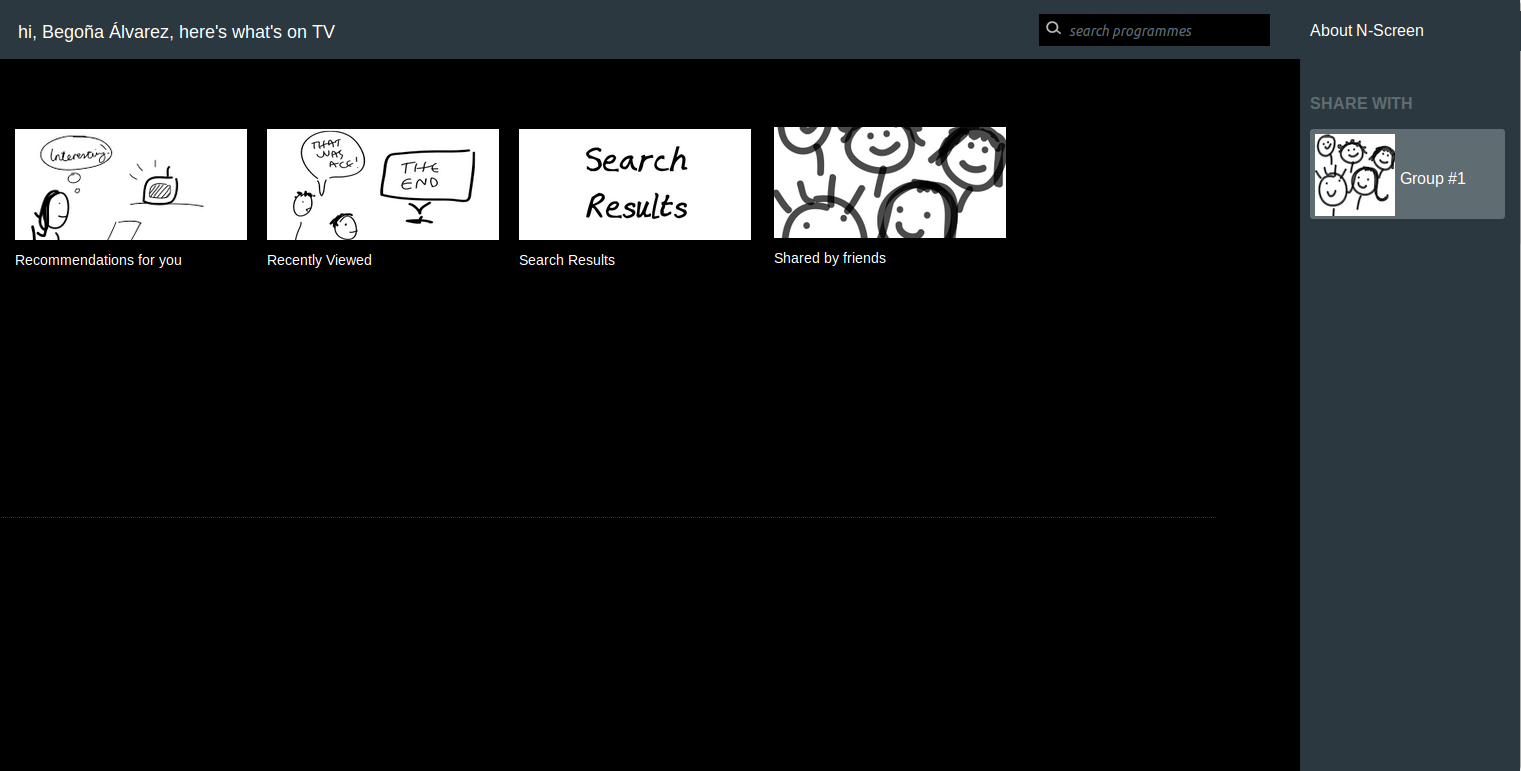
\epsfig{file=images/old_nscreen_homepahe.png, height=2in, width=3.5in}
\caption{Notube N-Screen Homepage}
\label{fig:oldhomepage}
\end{figure}

Consequently, we decided to display the homepage providing further information meanwhile trying to not disturb the user\cite{colborne2010simple}\cite{krug2014don}\cite{norman2002design}. We opted following the homepage design of \texttt{http://nscreen.notu.be/ted/} due to its simplicity and at the same time its further information provided \cite{nielsen2002homepage}. Figure \ref{fig:newhomepage} shows the result of our implemented homepage. 

\begin{figure}[!htb]
\centering
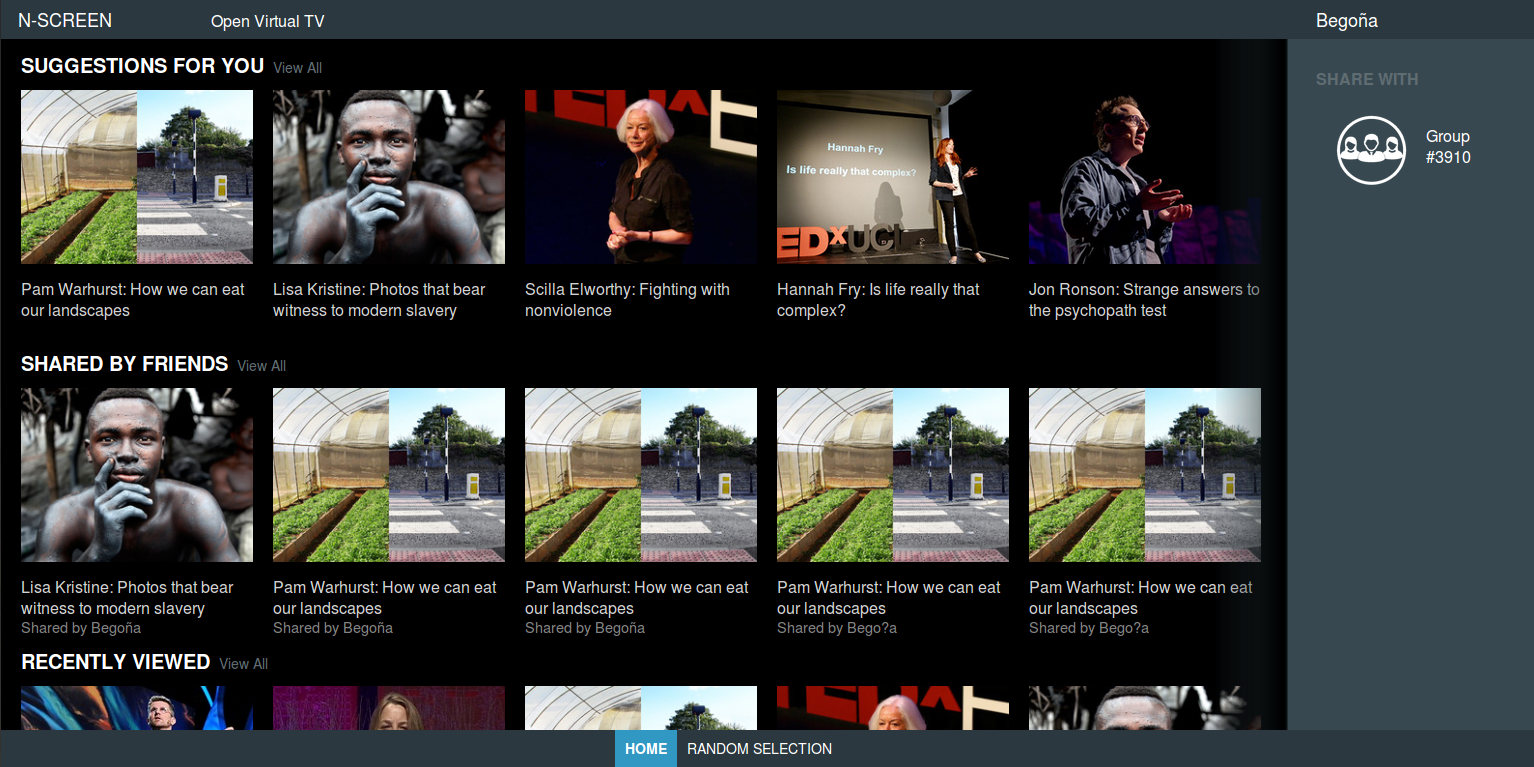
\epsfig{file=images/new_homepage.png, height=2in, width=3.5in}
\caption{New N-Screen Homepage}
\label{fig:newhomepage}
\end{figure}

Concerning channels replacement, the new design shows for every channel as 'Suggestions for you' or 'Shared by friends' a first sight view of five programmes -or less if the screen has a smaller size -. Furthermore, it has been added the possibility to view all the programmes contained with the addition of a clickable 'View All' next to the channel title. Figure \ref{fig:viewallzoom} shows this addition and Figure \ref{fig:viewallafter} shows the result after clicking 'View All' for one of the channels. 

\begin{figure}[!htb]
\centering
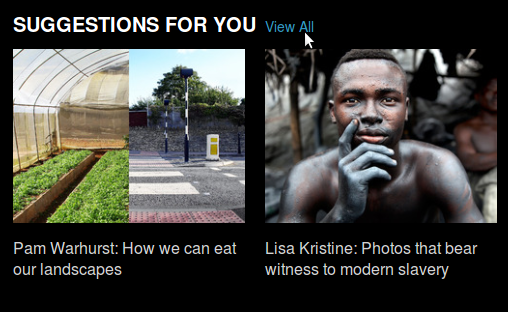
\epsfig{file=images/view_all_possibility_zoom.png, height=2in, width=3.5in}
\caption{View All Addition next to a Channel Title,New N-Screen Homepage}
\label{fig:viewallzoom}
\end{figure}

\begin{figure}[!htb]
\centering
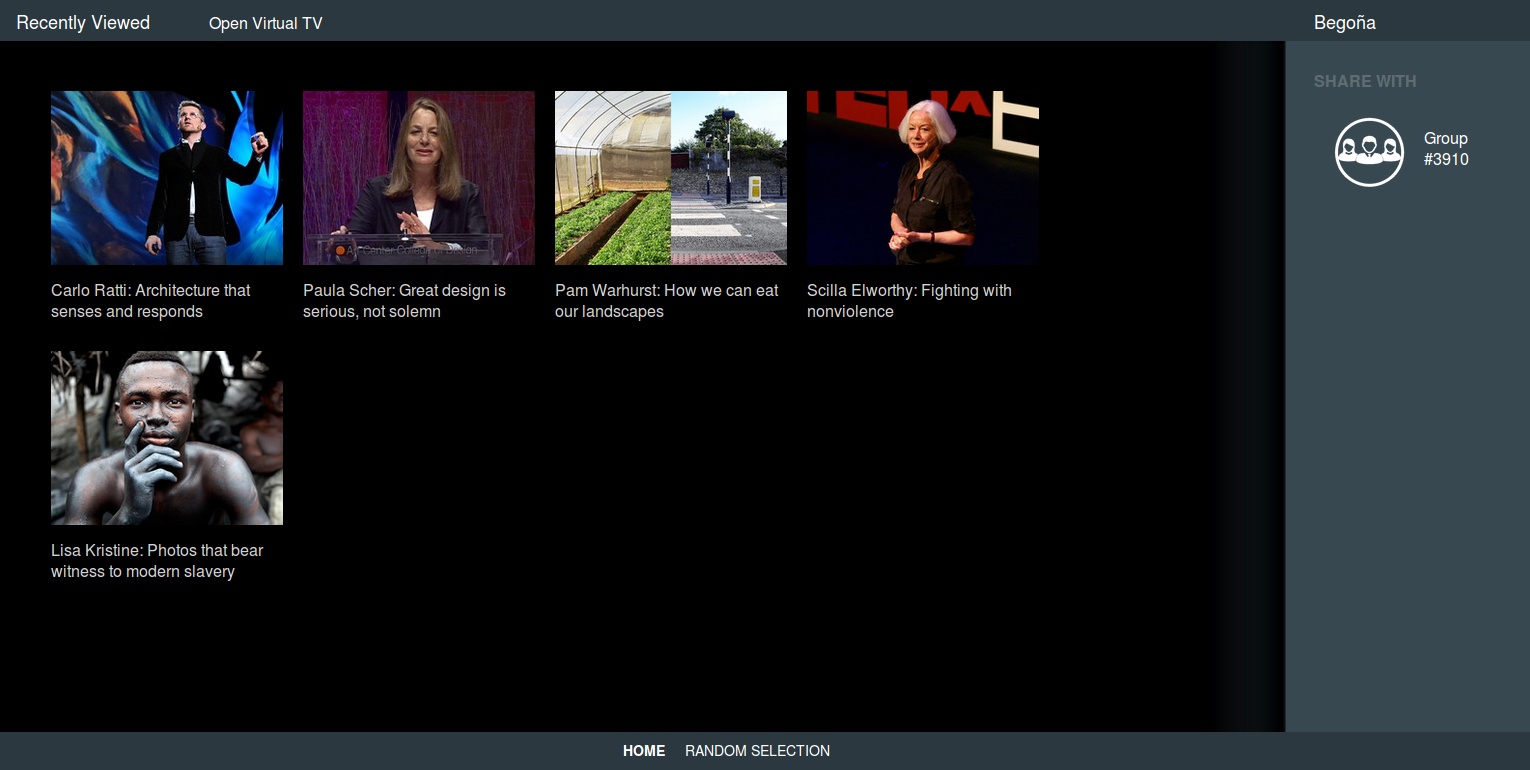
\epsfig{file=images/viewallclick.png, height=2in, width=3.5in}
\caption{Programmes Visualization after 'View All' click,New N-Screen}
\label{fig:viewallafter}
\end{figure}

Every channel contained in the new N-Screen homepage -Suggestions for You, Shared By Friends, Recently Viewed, Watch Later, Likes and Dislikes - present the same design approach. 

In addition, it has been implemented more design improvements concerning the homepage aesthetics. Most of the websites are currently showing information related to the user profile in the header at the right side\cite{colborne2010simple}\cite{krug2014don}\cite{norman2002design}. For this reason, the name of the user has been moved in the header from the left to the right side in order to maintain its placement customary. Moreover, the images places next to group number and members of the same group been redesigned, see Figure \ref{fig:roster}. 

\begin{figure}[!htb]
\centering
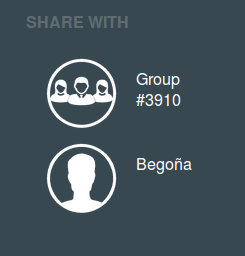
\epsfig{file=images/roster.png, height=1in, width=1in}
\caption{Images Redesign in Vertical-Right Bar,New N-Screen}
\label{fig:roster}
\end{figure}

\subsubsection{Selected Programme}

One of the most tedious parts during the design has been re-designing the visualization of a selected programme. During this phase, aesthetics and usability have been the most important factors. It has been included a vertical-right interactive bar next to the programme default image, see Figure \ref{fig:selectedprogramme}. This bar contains a set of five icons: Watch Later, Like, Dislike, Shared by Friends and Recently Viewed. It is important to mention that three of this icons -Watch Later, Like and Dislike- are call-to-action icons, which means that if the user clicks on one of them, the programme will be automatically added to the personal list which name is that precise icon. It is important to mention that if a programme is contained in one of the personal lists, the icon will be automatically rendered to be displayed in a different colour, as reminder for the user, see Figure \ref{fig:colouredicons}. 

\begin{figure}[!htb]
\centering
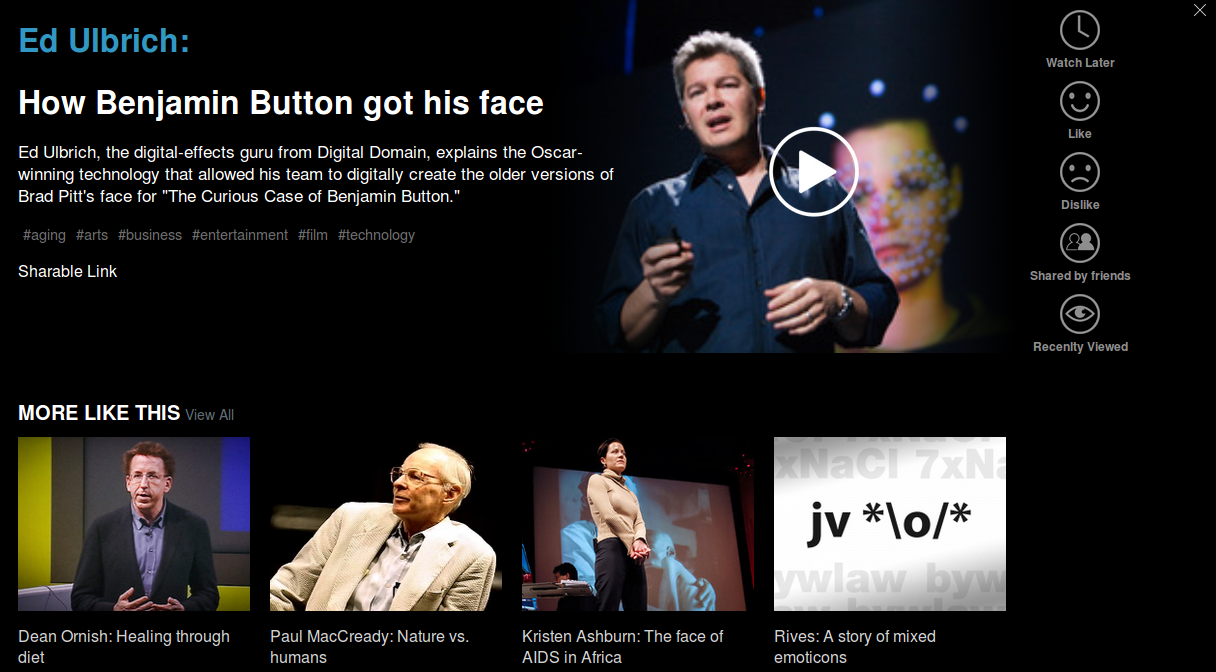
\epsfig{file=images/selected_programme.png, height=2in, width=3.5in}
\caption{Select Programme Visualization,New N-Screen}
\label{fig:selectedprogramme}
\end{figure}

\begin{figure}[!htb]
\centering
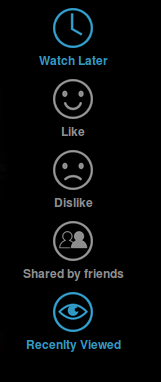
\epsfig{file=images/colouredicons.png, height=1in, width=0.5in}
\caption{Example of Coloured Icons,New N-Screen}
\label{fig:colouredicons}
\end{figure}

Additionally, it has been added below a programme description an inline set of hyperlinked tags extracted for the programme metadata, see Figure \ref{fig:tags}. A user can click to a desired tag to explore further related programmes. Figure \ref{fig:tagsclick} show the visualization of this action. 

\begin{figure}[!htb]
\centering
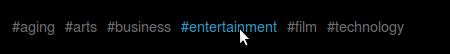
\epsfig{file=images/tags.png, height=0.5in, width=3in}
\caption{Hyperlinked Tags,New N-Screen}
\label{fig:tags}
\end{figure}

\begin{figure}[!htb]
\centering
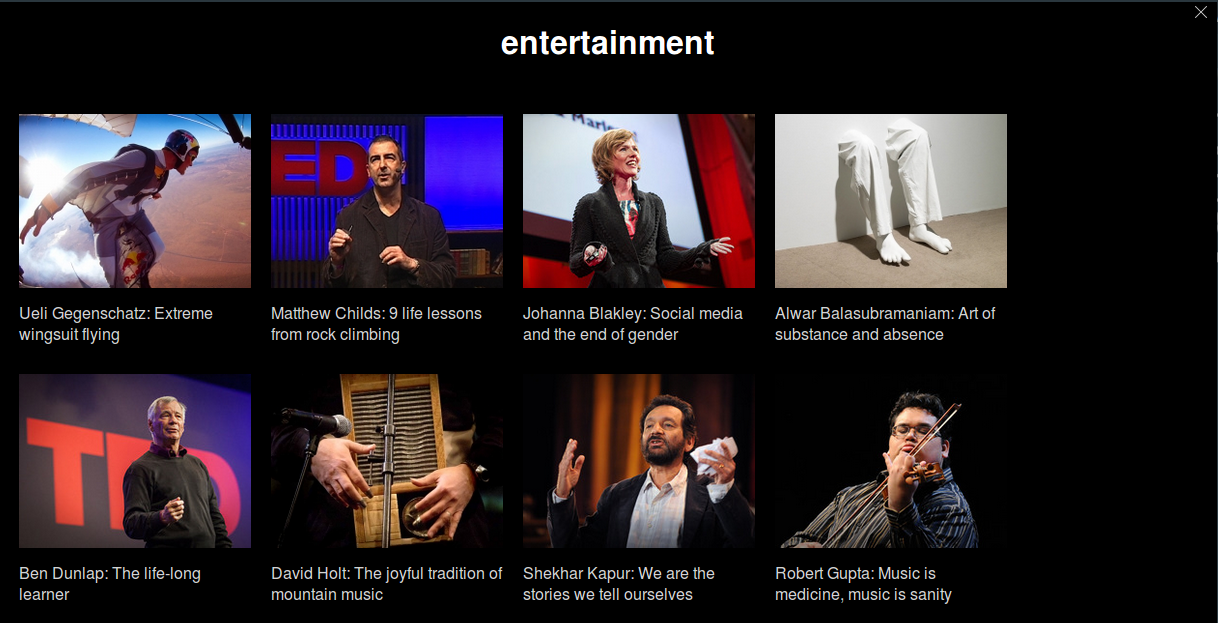
\epsfig{file=images/tagsclick.png, height=2in, width=3.5in}
\caption{Visualization of related programmes after the selection of a tag,New N-Screen}
\label{fig:tagsclick}
\end{figure}

At last, it has been included a clickable selection of related programmes below its summary, placed on the 'More Like This' section. 

\section{Evaluation and Results}
Initially, some tests were applied to the final platform for the purpose of proving its
proper functionality. The main features that make the platform valuable such as
registration, personal lists updating, sharing to a faraway user and remote TV have been tested. Afterwards, when the functionalities were demonstrated to work, an evaluation of the user experience has been carried out. The descriptions of
the tests and corresponding results are exposed in this section.

\subsection{Technical Tests}
This tests tried to prove that every functional part included in the source code was working. The test was carried out by ourselves and we tested the following features:

\begin{itemize}
  \item Registration 
  \begin{itemize}
  	\item [-]Username not already taken by another user
  	\item [-]Double entering password
  	\item [-]OpenID authorization
  	\item [-]Database members table initialization
  	\item [-]Database content table initialization
  	\item [-]Cache
  \end{itemize}
  \item Login
  \begin{itemize}
  	\item [-]Username and corresponding password
  	\item [-]OpenID authorization
  	\item [-]Security
  	\item [-]User personal row in database members table
  	\item [-]User personal row in database content table
  	\item [-]Database content table initialization
  	\item [-]Cache
  \end{itemize}
  \item Homepage 
  \begin{itemize}
  	\item [-]Content
  	\item [-]Channels - Personal Lists
  	\item [-]View All
  	\item [-]Shared by in Shared by Friends
  	\item [-]Random Selection
  	\item [-]User name
  	\item [-]Group number
  	\item [-]Group member names
  	\item [-]Drag\&Drop
  	\item [-]Virtual TV
  \end{itemize}
  \item Personal Lists Update
  \begin{itemize}
  	\item [-]Shared by Friends
  	\item [-]Recently Viewed
  	\item [-]Watch Later
  	\item [-]Likes
  	\item [-]Dislikes
  \end{itemize}
  \item Call-to-Action icons
  \begin{itemize}
  	\item [-]Watch Later
  	\item [-]Like
  	\item [-]Dislike
  \end{itemize}
  \item Non-Call-to-Action icons
  \begin{itemize}
  	\item [-]Shared by Friends
  	\item [-]Recently Viewed
  \end{itemize}
  \item Faraway Programme Sharing to a Single User
  \begin{itemize}
  	\item [-]Unique notifications
  	\item [-]Unique Shared by friends channel
  \end{itemize}
  \item Faraway Programme Sharing to a Group
  \begin{itemize}
  	\item [-]Group Notifications
  	\item [-]Group Shared by friends channel
  \end{itemize}
  \item Programme selection
  \begin{itemize}
  	\item [-]Information displayed
  	\item [-]Local play
  	\item [-]Call-to-action icons
  	\item [-]Tags
  	\item [-]More Like this
  \end{itemize}
  \item Virtual TV
  \begin{itemize}
  	\item [-]Sharing
  	\item [-]Play
  \end{itemize}
\end{itemize}

After the test we ascertained that every part listed above was correctly working. 
\subsection{User Experience Evaluation}
To accomplish the success of our platform, it was necessary to consider testing its interface as 
well. An interface is the intermediary between users and content. It guides them through different complexities found on an interactive web system. ''The happy marriage of architecture and interface--of logical structure and visual meaning--creates a cohesive user experience''\cite{fleming1998web}. 

In order to test this important part of the platform, we carried out a user experience (UX) evaluation in order to extract how users feel during the interaction. For this purpose, we recruited 5 participants: three women and two man across a spread of ages between 20 and 31. All participants descriped themselves as screen devices enthusiasts, regulary spending at least 2 leisure hours a day in front of a screen. 

Following some introductory context about our N-Screen in general, during each session we showed the participants our own version of N-Screen, containing a set of videos provided by TED Talks API, and we walked them through a group.watching scenario -with the author of this report taking the role of the participant's N-Screen 'friend'-. 

During the evaluation, we asked the participant to think out loud to extract their thoughts and feelings about our own N-Screen. The results of this evaluation are exposed in the following subsections. 

\subsubsection{Registration \& Login}

Each participant was required to sign up in our platform. Concerning the registration activity, all participants except one did not give importance to this step. This one participant required to be able to get into the platform without registration and sign up afterwards, if wanted. In addition, three participants selected the OpenID registration explaining that the one-click was actually much easier. Contrary, one of the participants selected the good registration due to lacking Facebook account. At last, the resting participant selected the good registration claiming a distrust sharing a personal social network profile.  

After registration, we required to every participant to sign in in order to test how intuitive was this process, since the registration pop-up appears before the log in option. No one showed any trouble to login.

\subsubsection{Homepage}

Each participant in an N-Screen group starts with a different set of personalised programme recommendations, and a set of empty personal lists -since they interaction just started-. We had to ask our participants to imagine these were based on their user profile. Despite this, all the participants liked the concept of seeing programme suggestions based on their own preferences.

All participants showed an enthusiastic feedback about the homepage. The display of a short set of videos below each channel was for them very informative and non disturbing. 

Additionally, tapping on a programme in our N-Screen displays an overlay with a brief programme synopsis with clickable tags, play button, a vertical bar containing call-to-action icons and a set of programmes related to the selected one. All participants showed a positive reaction to this overlay, considering it with the precise information needed. We asked the participants to try to interact with the programme overlay, and all of them found out easily that 'Watch Later', 'Like' and 'Dislike' buttons where clickable and concerned an updating of their personal lists, and also all of them realised that 'Shared by Friends' and 'Recently Viewed' were static buttons automatically rendered by the platform. Concerning the hyperlink metadata, all participants figured out that they were also clickable and were appreciative about them, showing videos related to a specific tag was very useful for everyone.  In addition, the play button was intuitive for every participant.  

It is important to mention that every participant except one exposed a comment without being asked about the random selection. They found this possibility definitely useful, since sometimes it is preferable to watch something totally non-related to own preferences and therefore find something new. 

A special test that we carried out was to ask to every participant to go back to home page if they were out of it. Every participant found out by themselves that there was a clickable button placed in the footer with the word HOME that could drive them there. 

At last, one of the participants showed disappointment with the navigation on the home page, preferring to be horizontally static and just allowing to scroll vertically. 
\subsubsection{Sharing \& Virtual TV}
 
During this phase of the test, we asked to all participants to share a program. One of the participants did not manage to accomplish it without a hint, three participants did it without trouble, and impressively the resting one starting sharing without even being asked to it, so for this last one was incredibly intuitive. 

Additionally, any problem to open the Virtual TV and drag \& drop something to it was showed, this last one since the previous phase provided a hint to accomplish the TV sharing.

All participants were very enthusiastic about the Virtual TV and found this featured extremely useful and innovative. ç

\subsubsection{General Overview}

At the end of the evaluation with every participant, we asked them how was their general feeling about the platform, how intuitive it was and also its aesthetic. Every participant shared a positive reaction after this questions, explaining that it was generally intuitive and also with a beautiful non disturbing minimalistic interface.  

\subsubsection{Results}
After the evaluation with final users, 
\section{Conclusions}
This paragraph will end the body of this sample document.
Remember that you might still have Acknowledgments or
Appendices; brief samples of these
follow.  There is still the Bibliography to deal with; and
we will make a disclaimer about that here: with the exception
of the reference to the \LaTeX\ book, the citations in
this paper are to articles which have nothing to
do with the present subject and are used as
examples only.
%\end{document}  % This is where a 'short' article might terminate

%ACKNOWLEDGMENTS are optional
\section{Acknowledgments}
This section is optional; it is a location for you
to acknowledge grants, funding, editing assistance and
what have you.  In the present case, for example, the
authors would like to thank Gerald Murray of ACM for
his help in codifying this \textit{Author's Guide}
and the \textbf{.cls} and \textbf{.tex} files that it describes.

%
% The following two commands are all you need in the
% initial runs of your .tex file to
% produce the bibliography for the citations in your paper.
\bibliographystyle{abbrv}
\bibliography{sigproc}  % sigproc.bib is the name of the Bibliography in this case
% You must have a proper ".bib" file
%  and remember to run:
% latex bibtex latex latex
% to resolve all references
%
% ACM needs 'a single self-contained file'!
%
%APPENDICES are optional
%\balancecolumns
\appendix
%Appendix A
\section{Headings in Appendices}
The rules about hierarchical headings discussed above for
the body of the article are different in the appendices.
In the \textbf{appendix} environment, the command
\textbf{section} is used to
indicate the start of each Appendix, with alphabetic order
designation (i.e. the first is A, the second B, etc.) and
a title (if you include one).  So, if you need
hierarchical structure
\textit{within} an Appendix, start with \textbf{subsection} as the
highest level. Here is an outline of the body of this
document in Appendix-appropriate form:
\subsection{Introduction}
\subsection{The Body of the Paper}
\subsubsection{Type Changes and  Special Characters}
\subsubsection{Math Equations}
\paragraph{Inline (In-text) Equations}
\paragraph{Display Equations}
\subsubsection{Citations}
\subsubsection{Tables}
\subsubsection{Figures}

\subsubsection{Theorem-like Constructs}
\subsubsection*{A Caveat for the \TeX\ Expert}
\subsection{Conclusions}
\subsection{Acknowledgments}
\subsection{Additional Authors}
This section is inserted by \LaTeX; you do not insert it.
You just add the names and information in the
\texttt{{\char'134}additionalauthors} command at the start
of the document.
\subsection{References}
Generated by bibtex from your ~.bib file.  Run latex,
then bibtex, then latex twice (to resolve references)
to create the ~.bbl file.  Insert that ~.bbl file into
the .tex source file and comment out
the command \texttt{{\char'134}thebibliography}.
% This next section command marks the start of
% Appendix B, and does not continue the present hierarchy
\section{More Help for the Hardy}
The acm\_proc\_article-sp document class file itself is chock-full of succinct
and helpful comments.  If you consider yourself a moderately
experienced to expert user of \LaTeX, you may find reading
it useful but please remember not to change it.
\balancecolumns
% That's all folks!
\end{document}
